\section{Date: 2024-10-16}
\noindent \textbf{Series ID: ATNHPIUS33140Q} 

\noindent This series is titled All-Transactions House Price Index for Michigan City-La Porte, IN (MSA) and has a frequency of Quarterly. The units are Index 1995:Q1=100 and the seasonal adjustment is Not Seasonally Adjusted.The observation start date is 1986-04-01 and the observation end date is 2024-04-01.The popularity of this series is 1. \\ 

\noindent \textbf{Series ID: DRALT100S} 

\noindent This series is titled Delinquency Rate on All Loans, Banks Ranked 1st to 100th Largest in Size by Assets and has a frequency of Quarterly, End of Period. The units are Percent and the seasonal adjustment is Seasonally Adjusted.The observation start date is 1985-01-01 and the observation end date is 2024-04-01.The popularity of this series is 26. \\ 

\subsection{Regression Tables and Plots}
\begin{center}
\begin{tabular}{lclc}
\toprule
\textbf{Dep. Variable:}              & value\_fred\_DRALT100S & \textbf{  R-squared:         } &     0.310   \\
\textbf{Model:}                      &          OLS           & \textbf{  Adj. R-squared:    } &     0.305   \\
\textbf{Method:}                     &     Least Squares      & \textbf{  F-statistic:       } &     67.73   \\
\textbf{Date:}                       &    Wed, 16 Oct 2024    & \textbf{  Prob (F-statistic):} &  8.12e-14   \\
\textbf{Time:}                       &        09:58:41        & \textbf{  Log-Likelihood:    } &   -289.22   \\
\textbf{No. Observations:}           &            153         & \textbf{  AIC:               } &     582.4   \\
\textbf{Df Residuals:}               &            151         & \textbf{  BIC:               } &     588.5   \\
\textbf{Df Model:}                   &              1         & \textbf{                     } &             \\
\textbf{Covariance Type:}            &       nonrobust        & \textbf{                     } &             \\
\bottomrule
\end{tabular}
\begin{tabular}{lcccccc}
                                     & \textbf{coef} & \textbf{std err} & \textbf{t} & \textbf{P$> |$t$|$} & \textbf{[0.025} & \textbf{0.975]}  \\
\midrule
\textbf{const}                       &       6.3015  &        0.376     &    16.750  &         0.000        &        5.558    &        7.045     \\
\textbf{value\_fred\_ATNHPIUS33140Q} &      -0.0204  &        0.002     &    -8.230  &         0.000        &       -0.025    &       -0.015     \\
\bottomrule
\end{tabular}
\begin{tabular}{lclc}
\textbf{Omnibus:}       & 22.326 & \textbf{  Durbin-Watson:     } &    0.035  \\
\textbf{Prob(Omnibus):} &  0.000 & \textbf{  Jarque-Bera (JB):  } &   27.308  \\
\textbf{Skew:}          &  1.012 & \textbf{  Prob(JB):          } & 1.18e-06  \\
\textbf{Kurtosis:}      &  3.431 & \textbf{  Cond. No.          } &     439.  \\
\bottomrule
\end{tabular}
%\caption{OLS Regression Results}
\end{center}

Notes: \newline
 [1] Standard Errors assume that the covariance matrix of the errors is correctly specified.

\begin{figure}
\centering
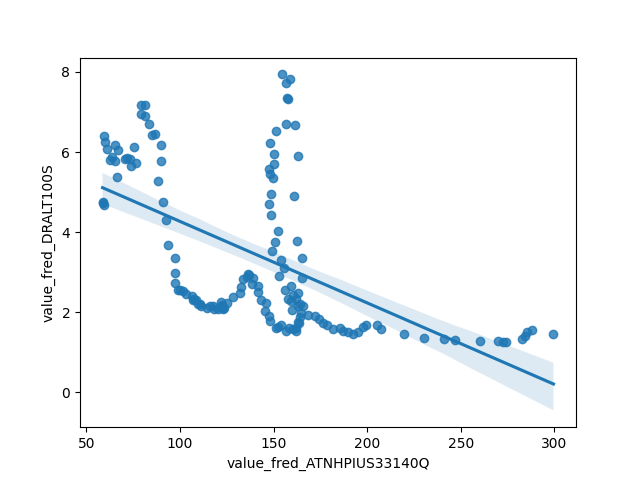
\includegraphics[scale = 0.9]{plots/plot_2024-10-16.png}
\caption{Regression Plot for 2024-10-16}
\end{figure}
\newpage
